\documentclass{article}
\usepackage{style} 
\usepackage{placeins}

%================
% Title and Author Information
%================

\title{{\titlefont \textbf{Title}} \\ {\large ETH Zürich\quad-\quad Autumn 2026}}
\author{Your Names & asdsf sdf & lsadjf asdf}
\date{\today}

\begin{document}
\maketitle % Renders the title page

\noindent\begin{tabular}{@{}llll}
    Authors & \theauthor \\
    E-Mails &  \href{mailto:yourname@student.ethz.ch}{yourname@student.ethz.ch} & \href{yourname@student.ethz.ch}{yourname@student.ethz.ch} & \href{yourname@student.ethz.ch}{yourname@student.ethz.ch} \\[6pt]
    Submission & \today
\end{tabular}

\linenumbers
%================
% Document Start
%================

\section{Introduction}
In this section, you should introduce the topic and context of your chosen study. Provide a brief description of the environmental event or process that you are focusing on, such as a specific flood, glacier or volcanic eruption. Explain where and when it occurred, and why it is of interest to you.

Clearly state the main objectives or research questions of your report.  This will help readers to understand the structure and scope of your work. Include your own hypotheses about the research questions. You do not need to include all the minor questions; just explain the purpose of the four main tasks on your exercise sheet.  This is how can cite papers or additional resources in text \cite{Bernhard2022} or \citep{DVN/OHHUKH_2018}.

\section{Methodology}
In this section, describe how you worked through the different tasks of your project. Outline the main steps you followed to analyse the satellite data in Google Earth Engine, for example, how you selected and filtered the images, which indices or masks you created, and how you extracted the information you needed.

Some tasks also ask you to explain how the Earth Observation systems you used actually work. In those cases, include a short explanation of the system you chose, what kind of sensor it uses (e.g. optical, radar, or thermal), what its spatial and temporal resolution is, and why it is a good fit for your analysis. The goal here is to make your approach understandable for someone who was not part of your group or had a different report topic.

\section{Results}
In this section, present the key results of your analysis. Include the maps, plots, and figures you created during your work. Try to structure the results in a logical order. You can for example make subsections for the different tasks.

If your project involves seasonal comparisons, you can use or adapt the layout shown in Figure~\ref{fig:seasonal_changes} to show changes over time using satellite imagery. Make sure all figures have good captions and are referred to in the text. You can also include screenshots or exports from your Google Earth Engine scripts. An example is shown in Figure~\ref{fig:gee_result}, but feel free to format and design your own visual outputs based on what fits your analysis best.

\begin{figure}[htbp!]
    \centering
    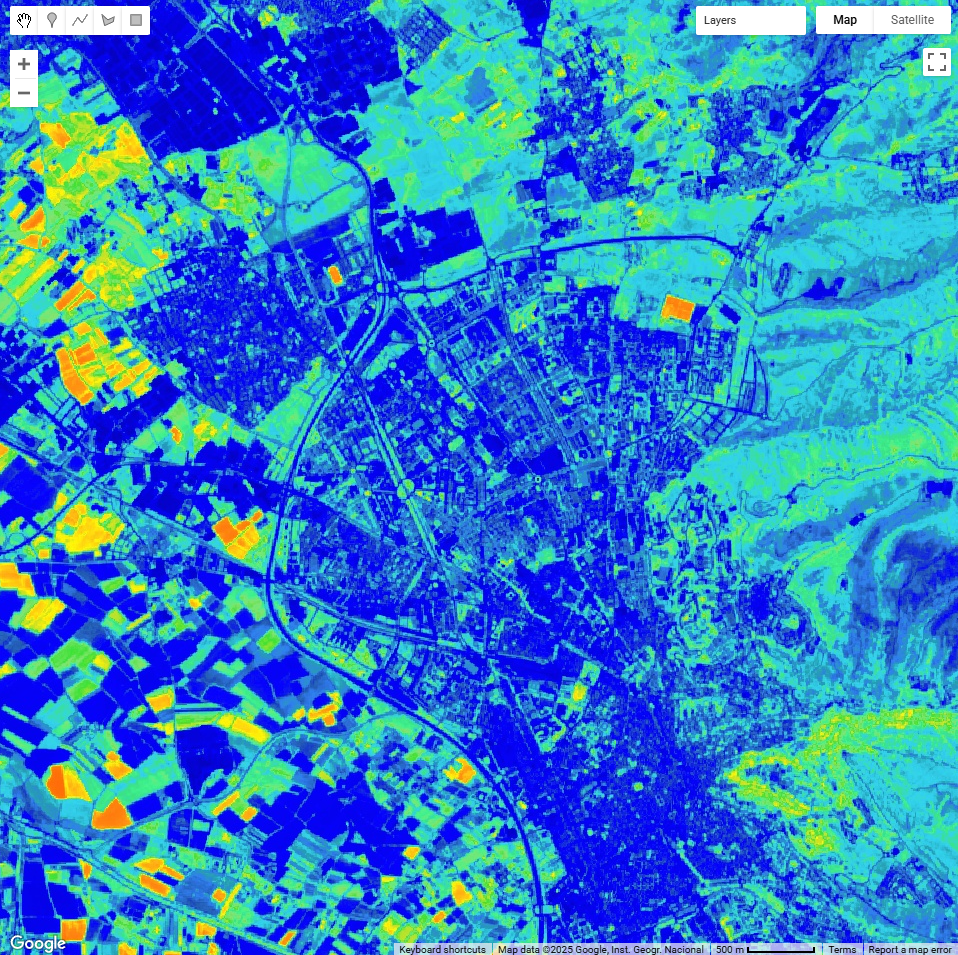
\includegraphics[width=0.4\textwidth]{Figures/NDVI_Granada.png}
    \caption{NDVI of the region around Granada, Spain, for the spring season (March–May) of 2023, derived from Sentinel-2 imagery using Google Earth Engine. The visualization uses a MODIS-style color palette to represent vegetation density.}
    \label{fig:gee_result}
\end{figure}


\begin{figure}[htbp!]
    \centering
    \begin{subfigure}[b]{0.24\textwidth}
        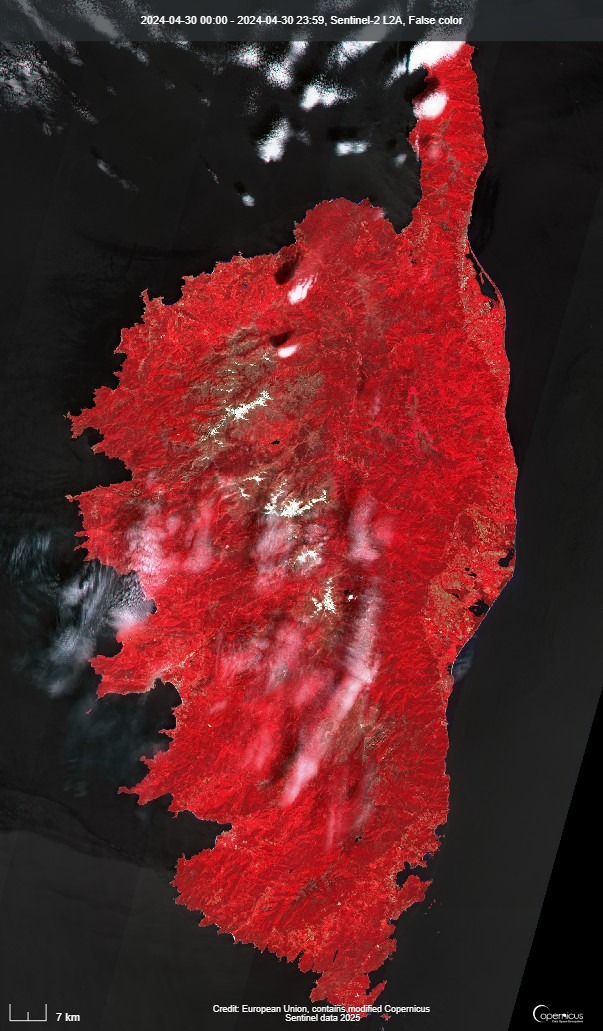
\includegraphics[width=\textwidth]{Figures/2024-04-30-00_00_2024-04-30-23_59_Sentinel-2_L2A_False_color.jpg}
        \caption{Spring}
        \label{fig:spring}
    \end{subfigure}
    \hfill
    \begin{subfigure}[b]{0.24\textwidth}
        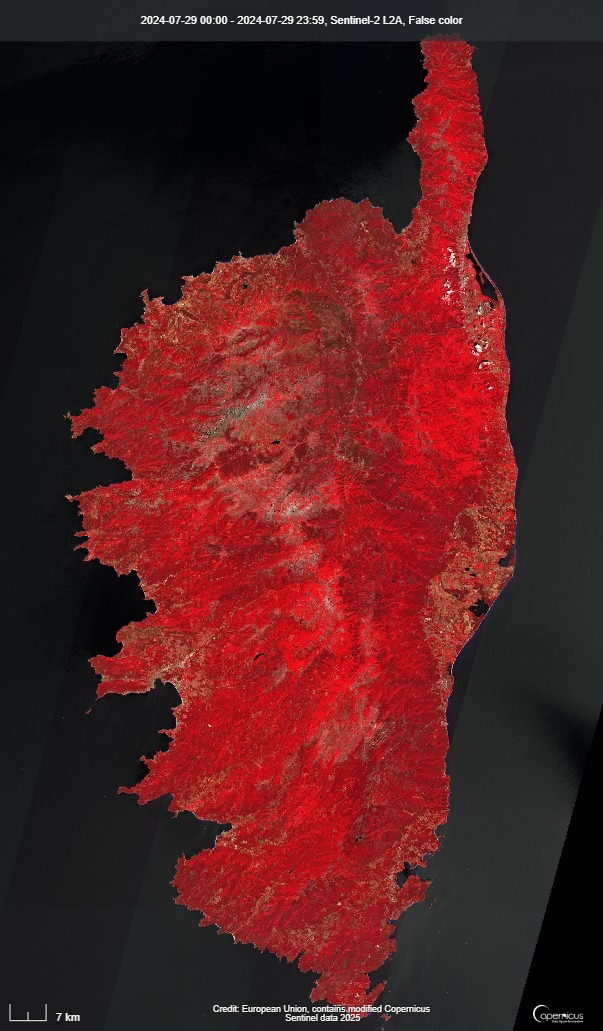
\includegraphics[width=\textwidth]{Figures/2024-07-29-00_00_2024-07-29-23_59_Sentinel-2_L2A_False_color.jpg}
        \caption{Summer}
        \label{fig:summer}
    \end{subfigure}
    \hfill
    \begin{subfigure}[b]{0.24\textwidth}
        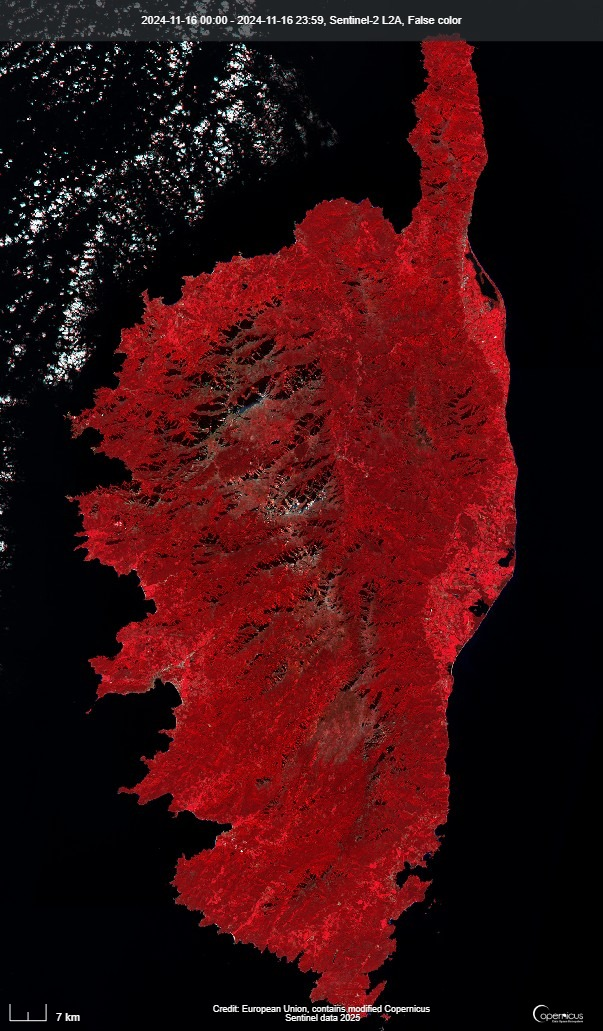
\includegraphics[width=\textwidth]{Figures/2024-11-16-00_00_2024-11-16-23_59_Sentinel-2_L2A_False_color.jpg}
        \caption{Autumn}
        \label{fig:autumn}
    \end{subfigure}
    \hfill
    \begin{subfigure}[b]{0.24\textwidth}
        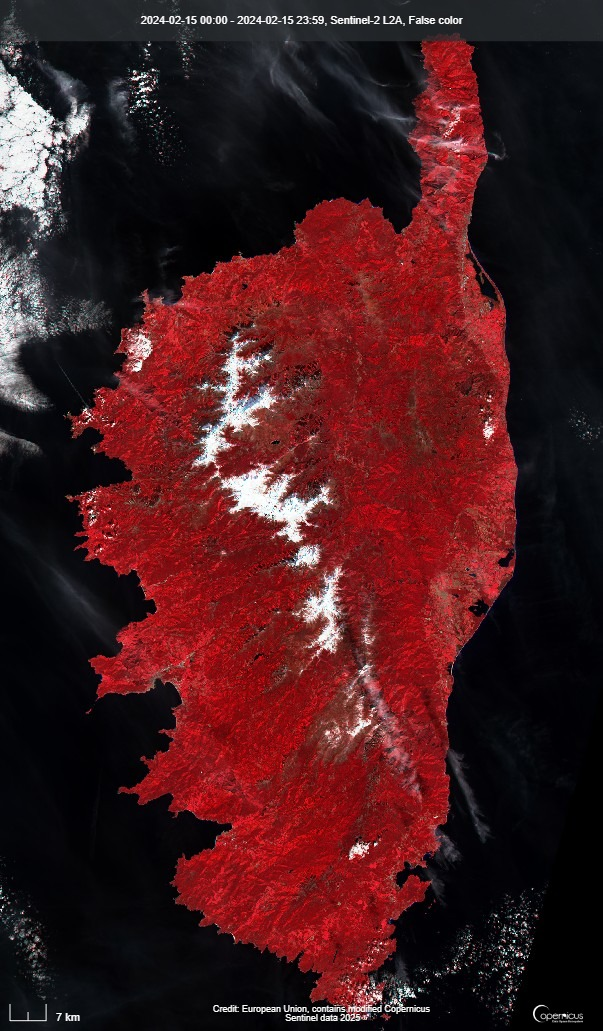
\includegraphics[width=\textwidth]{Figures/2024-02-15-00_00_2024-02-15-23_59_Sentinel-2_L2A_False_color.jpg}
        \caption{Winter}
        \label{fig:winter}
    \end{subfigure}
    \caption{False-color satellite imagery over Corsica from the Copernicus EO Browser. Images show seasonal variations using near-infrared composites for: (a) Spring, (b) Summer, (c) Autumn, and (d) Winter.}
    \label{fig:seasonal_changes}
\end{figure}


\section{Discussion and Conclusion}
Based on your results, discuss what they reveal about the environmental event or process you analysed. Were your initial research questions and hypotheses confirmed? Point out any unexpected patterns, uncertainties, or limitations in your analysis,for example, issues with data quality, sensor characteristics, or classification accuracy.

Try to connect your findings to a broader context. How do they compare with previous studies or official sources? What are the implications of your observations for understanding natural hazards, climate-related changes, or land cover dynamics?

To wrap up your report, summarise the key takeaways of your project. Highlight the most important results, how they contribute to answering your research questions, and what you learned during the process.

You may also suggest how the analysis could be improved in future work, for example, by using additional data, trying different methods, or applying the same approach to another region or time period.


\bibliographystyle{apalike-ejor}
\bibliography{references.bib}

\section*{Appendix}

\subsection{Source code}

Link to Github / Google Colab. Is a Google Colab actually needed or is Github fine??

\subsection{Use of generative artificial intelligence}

\begin{table}[h]
    \caption{Use of generative AI}
    \label{tab:AI_Use}
    \centering
    \begin{tabular}{llll}
    \toprule
    \makecell[l]{Artificial\\Intelligence} & Use & Scope & Comments \\
    \midrule
    Claude Sonnet 5.5 & Help with coding & Python modules & \href{https://claude.ai/share/8e2d447e-3fdb-4f93-a751-2df9f7116bd0}{Chat Link} \\
    \bottomrule
    \end{tabular}
\end{table}


\end{document}